\documentclass[twocolumn,10pt]{jarticle}
\setlength{\columnsep}{3zw}


\usepackage[dvipdfmx]{graphicx}

\graphicspath{{./image/}}

\title{楽器演奏におけるテンポ加速現象の解明}

\author{奥屋 直己}

\usepackage[height=26cm,width=16cm]{geometry}

\begin{document}

\maketitle

\section{はじめに}
音楽の演奏において、テンポを一定に保ち続けることは最も重要なことの一つである。しかし、演奏者の意図にかかわらずにテンポ変化が生じることがあり、そのような場合の多くは、テンポが加速する方向に変化する。このような意図しないテンポ変化は、演奏者の間で「走る」という表現で共有され、だれもがよく経験する現象である.「走る」ことは,事前に計画した表現の意識が弱まることや,合奏での演奏者間同期を妨げる要因となり,好ましくない現象とされる.この「走る」現象の原因としては,演奏者の心理的影響(不安や緊張,興奮など)が指摘されることが多いが,原因は定かではない.

Collyer \cite{Collyer}は,はじめはメトロノームと同期してレバーを押し,メトロノームが停止した後も同じテンポでレバー押しを継続する課題(同期継続課題:synchronization-continuation task)を用いた実験を報告している.彼は,27種類の目標テンポ条件(タッピング間隔として,175-825 msの範囲,テンポとして73-343 bpm)において同期継続課題を被験者に課し,テンポが遅くなりがちなテンポ帯と速くなりがちなテンポ帯があることを見出している.これによると,タッピング間隔が250-413 msおよび513-748 ms(80-117,145-240 bpm)の範囲でテンポが加速しやすく,それ以外の範囲では減速しやすかったという.さらに,永島氏と阪口氏 \cite{Nagasima}はリズムや強弱といった実際の音楽演奏に含まれるリズムパタンでの同期継続課題を用いた実験を報告している.彼らは図\label{Nagasima}の12種類(aは統制条件)のリズムパタンにおいて,130 bpmのテンポで同期継続課題を被験者に課した.その結果,リズムパタンの異なるExpt.1では条件cおよびeで安定的にテンポが減速した.アクセントパタンが異なるExpt.2では条件bでテンポの加速,条件gでテンポの減速がみられ(条件c,dでも加速傾向がみられたが,被験者のばらつきが大きかった),リズムパタンや強弱パタンがテンポ維持に影響を及ぼすことがわかったという.しかし、ほとんどが同期継続課題や主観的等価点から得たデータに焦点を当てており、同期継続課題中の指の動き方などの身体に焦点を当てたものは少ない。

身体の動きはテンポを一定に保つための何らかの基幹に影響を与える事が考えられる.岡野氏の報告 \cite{Okano}によれば,2人同時に同期継続課題を行った際に,一人で同期継続課題を行った時に比べて,テンポが速くなりやすいことが示唆されている.この2人の間での相互作用は,身体の動きと被験者内のテンポを一定に保つための基幹の間で1人でも起こり得るのではないかと考える.つまり,身体の動き,例えば腕を大きくうごかした際に比べ小さく動かした際では,リズムを一定に保つための基幹への影響が小さく,よりテンポを一定に保てるのではないかと考える.古屋氏 \cite{Huruya}は,ピアノでオクターブ連打をする際に,上肢の各部位の運動域およびその速度は,音量の増大に伴って増加するが,テンポの増加に対しては肘の最大角速度を除いて減少することを示唆している.これらのことから,同期継続課題においてタッピング間隔の短い音符(8分音符など)を含むリズムパタンで計測を行った際に,テンポ変化が起きづらいはずである.このことは永島氏と坂口氏 \cite{Nagasima}の報告から図\label{Nagasima}のExpt.1のf,gでテンポ変化が起きなかったことと一致する.またアクセントを含むリズムパタンでは,アクセント時に腕を大きく振り上げたことが予測され,この場合テンポは加速するはずであり図\label{Nagasima}のExpt.2のb,c,dで加速傾向がみられたこととも一致する.

以上のことから、本実験ではリズムパタンとアクセントパタンを伴うタッピングの同期継続課題に対して,タッピングする腕の振り上げ幅がテンポ維持特性に与える影響を実験的に検討した.具体的には,被験者に2種類のリズムパタンを「何も指示しない場合」「腕を大きく振り上げるよう指示した場合」「腕を小さく振り上げるよう指示した場合」の3種類の合計6種類を対象として,約2分間のテンポ維持課題を課し,テンポ変化の様子を計測した.
\begin{figure}
  \centering
  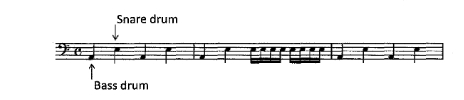
\includegraphics[width=6cm]{Arao_f1.jpg}
  \caption{The phrase with subdivisions of veats used in the experiment\cite{Arao}.}
  \label{Arao_f1}
\end{figure}
\begin{figure}
  \centering
  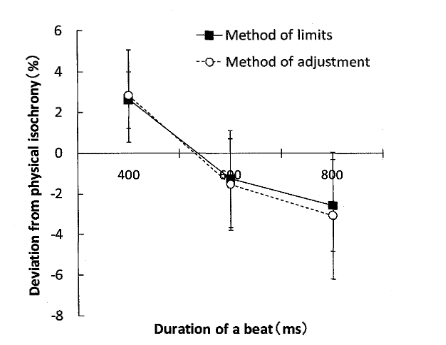
\includegraphics[width=6cm]{Arao_f2.jpg}
  \caption{Deviation from physical isochrony as a function og the duration of a beat in the ecperiment using phrases with subdivisions.Eroor bars represent 95\% confidence intervals\cite{Arao}.}
  \label{Arao_f2}
\end{figure}
\begin{figure}
  \centering
  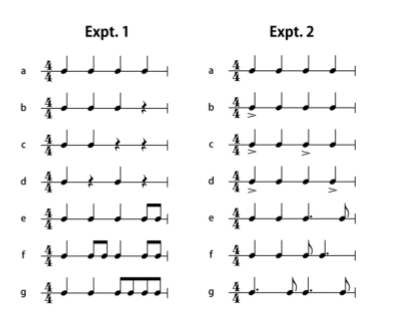
\includegraphics[width=6cm]{Nagasima.jpg}
  \caption{実験で用いたリズムパタン\cite{Nagasima}.}
  \label{Nagasima}
\end{figure}

\section{実験方法}
\subsection{被験者}
本実験には10名(男性○、女性○)の被験者が参加した。楽器演奏経験の乏しい被験者では安定したリズムパタンの再生が困難である場合が多いため、本実験の被験者には何らかの楽器演奏経験がある被験者のみを対象に行った。被験者には謝礼として、図書カード1000円分を手渡した。

\subsection{装置}
%もっと具体的に書く(どこにどう設置するかとか)
被験者のタッピング動作の記録には、Arduinoに圧力センサ、赤外線距離センサを組み合わせたスイッチを用いる。被験者はこのスイッチを手で叩くことにより計測する。Arduino上でUSBケーブルを介してシリアル通信をデータ転送レート9600 bpsで行い、計測PC上でProcessingにて作成したプログラムに随時転送し、テキストファイルとして出力した。時間はサンプリング周波数から割り出した値を後から追加した。同期時の基準テンポとしてはメトロノーム音源をmp3形式のファイルとして作成し、Arduino DFPlayerにて計測開始から24拍(4分の4拍子で8小節)のみ再生した。再生にはスピーカー(なんかのやつ)を使用し、被験者ごとに快適な音量に調節した。

\subsection{課題}
本実験には、従来の研究と同様に同期継続課題を用いた.従来の研究と異なる点は,被験者に腕の振り上げ方を指示した点である.本実験では,同期区間を16拍分(4分の4拍子で4小節)の8秒、継続区間を120拍分(4分の4拍子で30小節)の1分とした.

本研究では、Collyerの報告 \cite{Collyer}においてテンポ変化が生じにくかった120 bpmを目標テンポに設定して目標リズム音を作成した。

測定時、被験者には椅子に座り、机上のスイッチをタッピングするように指示した。タッピングをする際に使用する腕は、被験者に左右どちらがタッピングを行いやすいか確認をとり、被験者が選んだ腕でタッピングを行ってもらった。なお、被験者には腕の疲労が溜まりにくいように、高さ7 cmのクッションを机上に設置し、肘から手首にかけてクッションにおいてもらい、手首を振り下ろす形でタッピングを行ってもらった。

\subsection{条件}
本実験では、タッピング間隔が一定である統制条件と、2種類のリズムおよびアクセントパタンでタッピングを行う条件を設けた。条件aは統制条件、b,cはそれぞれ永島氏と坂口氏 \cite{Nagasima}の報告から,テンポ変化が起きなかったリズムパタンとテンポが安定的に加速したアクセントを含むリズムパタンである。

\subsection{手続き}
実験で使用するリズムに慣れるために、各リズムを使用した実験を行う前に、そのリズムで同期区間8小節、継続区間8小節の練習課題を課した。被験者がリズムパタンを理解し、タッピングできることを確認した後、同期区間 32拍分、継続区間 320拍分の本試験を行った。1試行に要した時間は2分弱である。したがって、実験全体で要した時間は、準備の時間も含めておよそ1時間だった。
\begin{center}
	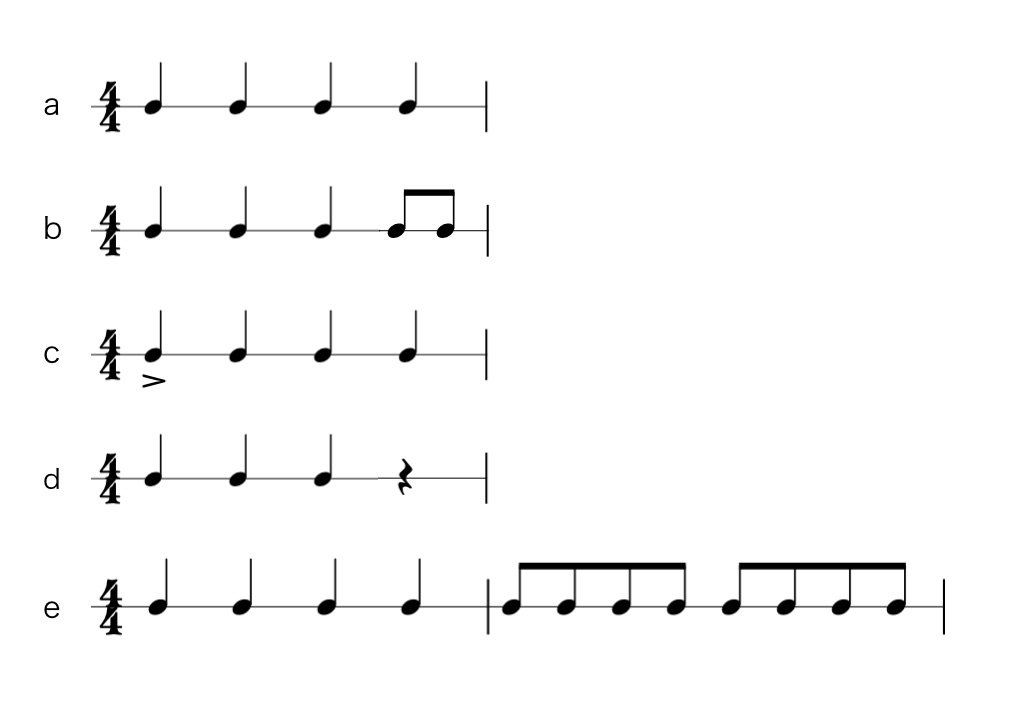
\includegraphics[width=5cm]{Rhythm_Pattern.jpg}
\end{center}	

\subsection{解析}
本実験の結果を統計的に検証するため、第2から第80までの各小節の小節長と第1小節の小節長との違いを順序尺度により検定した。

\bibliography{design}
\bibliographystyle{junsrt}

\end{document}
